\documentclass{book}
\usepackage{amsmath,amssymb,amsthm}
\usepackage{geometry}
\usepackage{graphicx}
\usepackage[colorlinks=true]{hyperref}
\usepackage{fancyhdr}
\usepackage{booktabs}
\usepackage{array}
\usepackage{multirow}
\usepackage{wrapfig}
\usepackage{float}
\usepackage{caption}
\usepackage{subcaption}
\usepackage{siunitx}
\usepackage{physics}
\usepackage{bm}
\usepackage{ctex}
\usepackage{unicode-math}
\usepackage{siunitx}

% 设置页面布局
\geometry{a4paper, left=25mm, right=25mm, top=25mm, bottom=25mm}

% 设置页眉页脚
\pagestyle{fancy}
\fancyhf{}
\fancyhead[RE]{\leftmark}
\fancyhead[LO]{\rightmark}
\fancyfoot[C]{\thepage}

% 定义定理环境
\newtheorem{theorem}{Theorem}[chapter]
\newtheorem{definition}[theorem]{Definition}
\newtheorem{example}[theorem]{Example}

% 设置标题格式
\title{量子化学}
\author{Ira N. Levine}
\date{第七版}

\begin{document}
	
	\maketitle
	
	\frontmatter
	\tableofcontents
	
	\mainmatter
	
	% ===== CHAPTER 1 =====
	\chapter{薛定谔方程}
	\section{量子化学}
	十七世纪末,艾萨克·牛顿(Isaac Newton)创立了\textbf{经典力学},即宏观物体的运动规律。二十世纪初,物理学家发现经典力学无法正确描述原子和分子的电子和原子核等极小粒子的行为。这类粒子的行为由一组称为\textbf{量子力学}的定律来描述。\\
	\indent \textbf{量子化学}将量子力学应用于化学问题。量子化学的影响在化学的各个分支中都很明显。物理化学家利用量子力学(借助统计力学)计算气体的热力学性质(如熵、热容量);解释分子光谱,从而通过实验确定分子性质(如分子几何形状、偶极矩、内旋转能垒、同分异构体之间的能量差异);从理论上计算分子性质;计算化学反应中过渡态的性质,从而估算速率常数;理解分子间作用力;以及处理固体中的成键问题。\\
	\indent 有机化学家利用量子力学估算分子的相对稳定性,计算反应中间产物的性质,研究化学反应的机理,以及分析和预测核磁共振谱。\\
	\indent 分析化学家广泛使用光谱法。只有利用量子力学,才能正确理解和解释光谱中的谱线频率和强度。\\
	\indent 无机化学家使用配体场理论(一种近似量子力学的方法)来预测和解释过渡金属络离子的性质。\\
	\indent 虽然重要生物分子的巨大尺寸使得对它们进行量子力学计算极其困难,但生物化学家们正开始从对生物分子构象、酶与底物结合以及生物分子溶解的量子力学研究中获益。\\
	\indent 量子力学决定了纳米材料(至少有一个维度在 1 nm到 100 nm之间的物体)的特性,目前正在开发处理纳米材料的计算方法。当材料的一个或多个尺寸小于 100 nm(尤其是小于 20 nm)时,其光学、电子、化学和其它特性就会发生与宏观材料显著不同的巨大变化。一个维度在 1 nm到 100 nm之间的半导体或金属物体称为\textit{量子阱};两个维度在此范围内的称为\textit{量子线};三个维度都在此范围内的称为\textit{量子点}。这些名称中的 “量子 ”一词表明量子力学在决定此类材料特性方面发挥了关键作用。许多人猜测,纳米科学和纳米技术将带来 “下一次工业革命”。\\
	\indent 计算机计算速度的迅速提高和分子计算新方法(如密度泛函理论-参见第 16.4 节)的发展,使量子化学成为化学各个领域的实用工具。现在,有几家公司出售用于分子量子化学计算的量子化学软件。这些软件不仅适用于量子化学家,也适用于其他各类化学家。由于量子化学及相关理论和计算方法的作用日益显著,美国化学学会于 2005 年开始出版新的期刊《化学理论与计算杂志》(Journal of Chemical Theory and Computation)。\\
	\indent “\textit{量子力学......几乎是所有现代科学技术的基础。它支配着晶体管和集成电路的行为......并且是......现代化学和生物学的基础。}”[斯蒂芬·霍金(Stephen Hawking),《时间简史》,1988 年,Bantam 出版社,第 4 章)]
	
	\section{量子力学的历史背景}
	\noindent 量子力学的发展起源于 1900 年普朗克(Planck)对加热固体发出的光的研究,因此我们首先要讨论光的本质。\\
	\indent 1803 年,托马斯·杨(Thomas Young)通过观察光穿过两个相邻针孔时的衍射和干涉,为光的波动性提供了令人信服的证据。(\textit{衍射}是波绕障碍物弯曲。\textit{干涉}是将两个频率相同的波结合在一起,产生一个波,该波在空间每一点的扰动是每个干涉波在该点产生的扰动的代数和或矢量和。参见任何一年级物理课本)。\\
	\indent 1864 年,詹姆斯·克拉克·麦克斯韦(James Clerk Maxwell)建立了四个方程,即麦克斯韦方程组(Maxwell'sequations),统一了电学和磁学定律。麦克斯韦方程预言:加速的电荷会以电磁波的形式辐射能量,电磁波由振荡的电场和磁场组成。麦克斯韦方程预测的这些波的速度与实验测得的光速相同。\\
	\indent 1888 年,海因里希·赫兹(Heinrich Hertz)根据麦克斯韦方程组的预测,探测到了电火花中加速电荷产生的无线电波。这使物理学家确信,光确实是一种电磁波。\\
	\indent 所有电磁波在真空中都以$c = 2.998 \times 10^8$ m/s的速度传播。电磁波的频率$\nu$和波长$\lambda$的关系是
	\begin{equation}
		\boxed{\lambda \nu = c}
	\end{equation}
	(方框内的等式应牢记;附录中给出了希腊字母表)。根据电磁波的频率,人们给电磁波进行了分类。按照频率递增的顺序依次为无线电波、微波、红外线辐射、可见光、紫外线辐射、X 射线和$\gamma$射线。我们用光来表示任何一种电磁辐射。可见光和紫外线辐射的波长以前用埃(\AA)来表示,现在用纳米(nm)来表示:
	\begin{equation}
		\boxed{1 \: \text{nm} = 10^{-9} \: \text{nm}, \qquad 1 \: \text{\AA}= 10^{-10} \: \text{m} = 0.1 \: \text{nm}}
	\end{equation}
	\indent 19 世纪 90 年代,物理学家测量了在固定温度下加热黑体发出的各种频率的光强度,并在多个温度下进行了这些测量。\textit{黑体}是一种能吸收落在其上的所有光线的物体。一种对黑体对良好近似是一个带有小孔的空腔。1896 年,物理学家维恩(Wien)提出了黑体辐射与光频和黑体温度的关系式:$I=a\nu^3/\text{e}^{b\nu /T}$,其中$a$与$b$是经验常数,$I \text{d} \nu$是黑体在单位时间和单位表面积内辐射的频率在$\nu$到$\nu + \text{d} \nu$范围内的能量,其中$\text{d} \nu$是一个无穷小的频率范围。维恩的公式很好地拟合了 1896 年的黑体辐射数据,但他对该公式的理论论证却不令人满意。\\
	\indent 1899-1900 年,对黑体辐射的测量扩展到了比以前更低的频率,维恩公式在低频下显示出较大的偏差。这些偏差促使物理学家马克斯·普朗克(Max Planck)于 1900 年 10 月提出了以下公式$I=a \nu^3 / \left(\text{e}^{b\nu / T}-1\right)$,并发现该公式适用于所有频率的数据。\\
	\indent 提出这个公式后,普朗克一直在寻找理论依据。1900 年 12 月,他向德国物理学会提交了他的公式的理论推导。普朗克假定黑体中的辐射发射器和吸收器是与空腔中的电磁辐射处于平衡状态的谐振电荷(“谐振子”)。他假设频率为$\nu$的谐振子的总能量由$N$个不可分割的 “能量元素”组成,每个能量元素的大小为$h\nu$,其中$N$为整数,$h$(普朗克常数)是物理学中的一个新常数。普朗克将这些能量元素分布在谐振子中。实际上,每个谐振子的能量必须是$h\nu$的整数倍(尽管普朗克没有明说)。因此,每个谐振子的能量都被量子化了,这意味着谐振子的能量只允许是某些分立的值。普朗克的理论导出了$a=2 \pi  h/c^2$和$b=h/k$,其中$k$是玻尔兹曼(Bolzmann)常量。通过拟合实验中得到的黑体辐射曲线,普朗克常数为$h=6.6 \times 10^{-34}$ J$\cdot$s。\\
	\indent 普朗克的工作通常被认为是量子力学的开端。然而,物理学史学家们一直在争论:1900 年的普朗克究竟是将能量量子化视为对物理现实的描述,还是仅仅将其视为一种数学近似,从而使他能够获得正确的黑体辐射公式。[见 O. Darrigol,Centaurus,43,219 (2001);C. A. Gearhart,Phys. Perspect.,4,170 (2002)(可在线查阅:employees.csbsju.edu/cgearhart/Planck/PQH.pdf;S. G. Brush,Am. J.Phys., 70, 119 (2002) (www.punsterproductions.com/~sciencehistory/cautious.htm).]。物理历史学家克拉格(Kragh)指出:“\textit{如果说 1900 年 12 月物理学发生了一场革命,似乎没有人注意到它。普朗克也不例外,赋予他的工作的重要性在很大程度上是一种历史重构。}”(H. Kragh,《物理学世界》,2000 年 12 月,第 31 页)\\
	\indent 能量量子化的概念与以往物理学的所有理念直接相悖。经典力学认为:物质体的能量可以连续变化。然而,只有在能量量子化的假设下,才能得到正确的黑体辐射曲线。\\
	\indent 能量量子化的第二个应用是\textit{光电效应}。在光电效应中,光照射到金属上会导致电子被激发。波的能量与其强度成正比,而与其频率无关。因此光的电磁波图象会让人想到:发射的光电子的动能会随着光强度的增加而增加,但不会随着光频率的变化而变化。\\
	\indent 1905 年,爱因斯坦(Einstein)指出:将光视为由粒子状实体(称为\textit{光子})组成的集合体,每个光子都具有能量
	\begin{equation}
		\boxed{E=h\nu}
		\label{eq:photoelectric effect equation}
	\end{equation}
	就可以解释这些观测结果。当金属中的电子吸收光子时,所吸收的光子能量的一部分被用来克服将电子固定在金属中的力,剩余的能量则转化为电子逸出后的动能。由能量守恒,有$h\nu = \phi+ T$,其中$\phi$是电子逸出金属表面所需的最小能量(金属的功函数),$T$是被激发电子的最大动能。提高光的频率$\nu$会增加光子能量,从而增加被激发电子的动能。增加固定频率下的光强度会增加光子撞击金属的速度,从而增加电子的发射速度,但不会改变每个发射电子的动能。(克拉格认为:“\textit{可以有力地证明,是爱因斯坦首先认识到了量子理论的本质。}”;H. Kragh,《物理世界》,2000 年 12 月,第 31 页)\\
	\indent 光电效应表明:除了在衍射实验中表现出波动性外,光还可以表现出粒子性。\\
	\indent 1907 年,爱因斯坦将能量量子化应用于固体元素中原子的振动。假设每个原子在每个方向$\left(x,y,z\right)$上的振动能量被限制为$h\nu_{vib}$的整数倍,其中振动频率$\nu_{vib}$是元素的性质。爱因斯坦利用统计力学推导出固体恒容热容$C_V$的表达式。他的公式与已知的钻石$C_V$与温度的关系数据相当吻合。\\
	\indent 现在我们来考虑物质的结构。\\
	\indent 19 世纪末,对放电管和自然放射性的研究表明:原子和分子是由带电粒子组成的。电子带有负电荷,而质子带有与电子电荷大小相等但符号相反的正电荷,其质量是电子的 1836 倍。原子的第三种成分-中子(1932 年发现)不带电荷,比质子稍重。\\
	\indent 从 1909 年开始,卢瑟福(Rutherford)、盖革(Geige)和马斯登(Marsden)反复将一束$\alpha$粒子穿过薄金属箔,并让它们落在荧光屏上,从而观察到粒子的偏转。$\alpha$粒子是从天然放射性衰变中获得的带正电荷的氦核。大多数$\alpha$粒子通过金属箔时基本上没有发生偏转,但令人惊讶的是,少数粒子发生了很大的偏转,有些粒子向后偏转。如果正电荷遍布整个原子[正如 J. J. 汤姆逊(Thomson)在 1904 年提出的那样],那么一旦高能$\alpha$粒子穿透原子,斥力就会减弱,根据经典静力学,在原子中心的斥力为零。因此,卢瑟福得出结论:只有当正电荷集中在一个微小而沉重的原子核中时,才会发生如此大的偏转。\\
	\indent 原子包含一个极小(半径为$10^{-13}$到$10^{-12}$ cm)的重核,由中子和$Z$个质子组成,其中$Z$是原子序数,原子核外有$Z$个电子,带电粒子的相互作用遵循库仑定律。(核子在原子核内通过强相互作用结合在一起,这与我们无关)原子的半径约为1 \AA,气体动力学理论的结果就表明了这一点。\\
	\indent 原子和分子的化学性质是由其电子结构决定的,因此就产生了电子运动和能量的性质问题。由于原子核的质量远大于电子,我们认为原子核的运动与电子的运动相比是微小的。\\
	\indent 1911 年,卢瑟福提出了原子的行星模型,其中电子以不同的轨道围绕原子核旋转,就像行星围绕太阳旋转一样。然而,这一模型存在一个根本性的难题。根据经典电磁理论,加速的带电粒子会以电磁波(光波)的形式辐射能量。以恒定速度围绕原子核旋转的电子正在被加速,因为其速度矢量的方向在不断变化。因此,卢瑟福模型中的电子应该不断地通过辐射损失能量,从而向原子核螺旋运动。因此,根据经典(19 世纪)的物理学,卢瑟福的原子结构是不稳定的,会发生坍缩。\\
	\indent 1913 年,尼尔斯·玻尔(Niels Bohr)将能量量子化的概念应用于氢原子,提出了解决这一难题的可行方法。玻尔假定氢原子中电子的能量是量子化的,电子只能在一系列允许的轨道中的一个轨道上运动。当电子从一个玻尔轨道过渡到另一个玻尔轨道时,一个频率$\nu$满足
	\begin{equation}
		\boxed{E_{upper}-E_{lower}=h\nu}
		\label{eq:Higher state to lower state delta energy}
	\end{equation}
	的光子被吸收或激发。其中$E_{upper}$和$E_{lower}$是高低两个状态的能量(能量守恒)。玻尔假定电子从自由(电离)态过渡到束缚轨道时会发射出一个光子,其频率是电子在束缚轨道中经典旋转频率的二分之一的整数倍,他利用经典力学推导出了氢原子能级的计算公式。利用\ref{eq:Higher state to lower state delta energy},他得到了与观测到的氢谱一致的结果。然而,用玻尔理论拟合氦光谱的尝试却失败了。此外,该理论无法解释分子中的化学键。\\
	\indent 玻尔模型的失败源于使用经典力学来描述原子中的电子运动。原子光谱显示出离散的频率,这表明只有某些能量的运动是允许的;以及电子能量是量子化的。然而,经典力学允许连续的能量范围。因此,路易斯·德布罗意(Louis de Broglie)在 1923 年提出:电子的运动可能具有波的一面。质量为$m$、速度为$v$的电子将具有波长
	\begin{equation}
		\lambda=\frac{h}{mv}=\frac{h}{p}
		\label{eq:de Brogile equation}
	\end{equation}
	其中$p$是线性动量。德布罗意通过与光子的类比推理得出公式\ref{eq:de Brogile equation}。根据爱因斯坦的狭义相对论,光子的能量可以用$E=pc$表示,其中$c$是光速,$p$是光子的动量。利用$E_{photon}=h\nu$可以得到光子以$c$的速度运动时的$pc=h\nu =hc/\lambda$和$\lambda = h/p$。方程式 \ref{eq:de Brogile equation} 是电子相应的方程式。\\
	\indent 1927 年,戴维森(Davisson)和格尔默(Germer)通过实验证实了德布罗意的假设,他们从金属中反射电子并观察到衍射效应。1932 年,斯特恩(Stern)在氦原子和氢分子中观察到了同样的效应,从而验证了波效应并非电子所特有,而是微观粒子运动的某种普遍规律的结果。通过衍射光栅可以观察到大至 C$_{48}$H$_{26}$F$_{24}$N$_8$O$_8$的分子的衍射和干涉现象	。[T. Juffmann 等,Nat. Nanotechnol.,7,297 (2012)]。有关分子干涉图案形成的影片,请访问 www.youtube.com/watch?v=vCiOMQIRU7I。\\
	\indent 因此,电子的行为在某些方面像粒子,而在另一些方面则像波。我们面临着物质(以及光)表面上自相矛盾的 “波粒二象性”。电子怎么可能既是粒子(局部实体),又是波(非局部实体)呢?答案是电子既不是波也不是粒子,而是另一种东西。用经典物理学的波或粒子概念来准确描述电子的行为是不可能的。经典物理学的概念是根据宏观世界的经验发展而来的,并不能正确描述微观世界。进化塑造了人类大脑,使其能够理解并有效处理宏观现象。人类神经系统的发展并不是为了处理原子和分子层面的现象,因此我们无法完全理解这些现象也就不足为奇了。\\
	\indent 虽然光子和电子都表现出明显的二元性,但它们并不是同一类实体。光子在真空中以$c$的速度运动,其静止质量为零;而电子始终具有$v<c$和非零静止质量。光子必须始终按相对论处理,但速度远小于$c$的电子可以按非相对论处理。
	
	\section{不确定性关系}
	让我们来看看波粒二象性对同时测量微观粒子的$x$坐标和线动量$x$分量的尝试有什么影响。我们从一束动量为$p$、沿$y$方向运动的粒子束开始,让粒子束落在一个窄缝上。狭缝后面是一块照相板。见图\ref{fig:1.1}。\\
	\indent 粒子通过宽度为$w$的狭缝时,其$x$坐标的不确定性为$w$。我们将这种$x$值的分布称为$\Delta x$,即有$\Delta x = w$。\\
	\indent 由于微观粒子具有波的特性,它们会被狭缝衍射,在平板上产生衍射图样(就像光束一样)。图 \ref{fig:1.1}中图形的高度表示到达给定点的粒子数量。衍射图样显示:当粒子被狭缝衍射时,它们的运动方向发生了改变,因此部分动量被转移到了$x$方向。动量在$x$方向上的分量$p_x$等于动量矢量$\overrightarrow{p}$在$x$方向上的投影。向上偏转$\alpha$角的粒子的动量满足$p_x=p\sin \alpha$;向下偏转$\alpha$角的粒子的动量满足$p_x=-p \sin \alpha$。由于大多数粒子的偏转范围在$-\alpha$到$\alpha$之间,其中$\alpha$是与衍射图样中第一个最小值的夹角,因此我们将以中心衍射峰中动量值的一般作为动量$x$分量不确定性$\Delta p_x$的量度:$\Delta p_x = p \sin \alpha$。\\
	\indent 因此,在狭缝处进行测量,有
	\begin{equation}
		\Delta x \Delta p_x = pw \sin \alpha 
		\label{eq:diffract equation on x}
	\end{equation}
	
	\begin{figure}[h!]
		\centering
		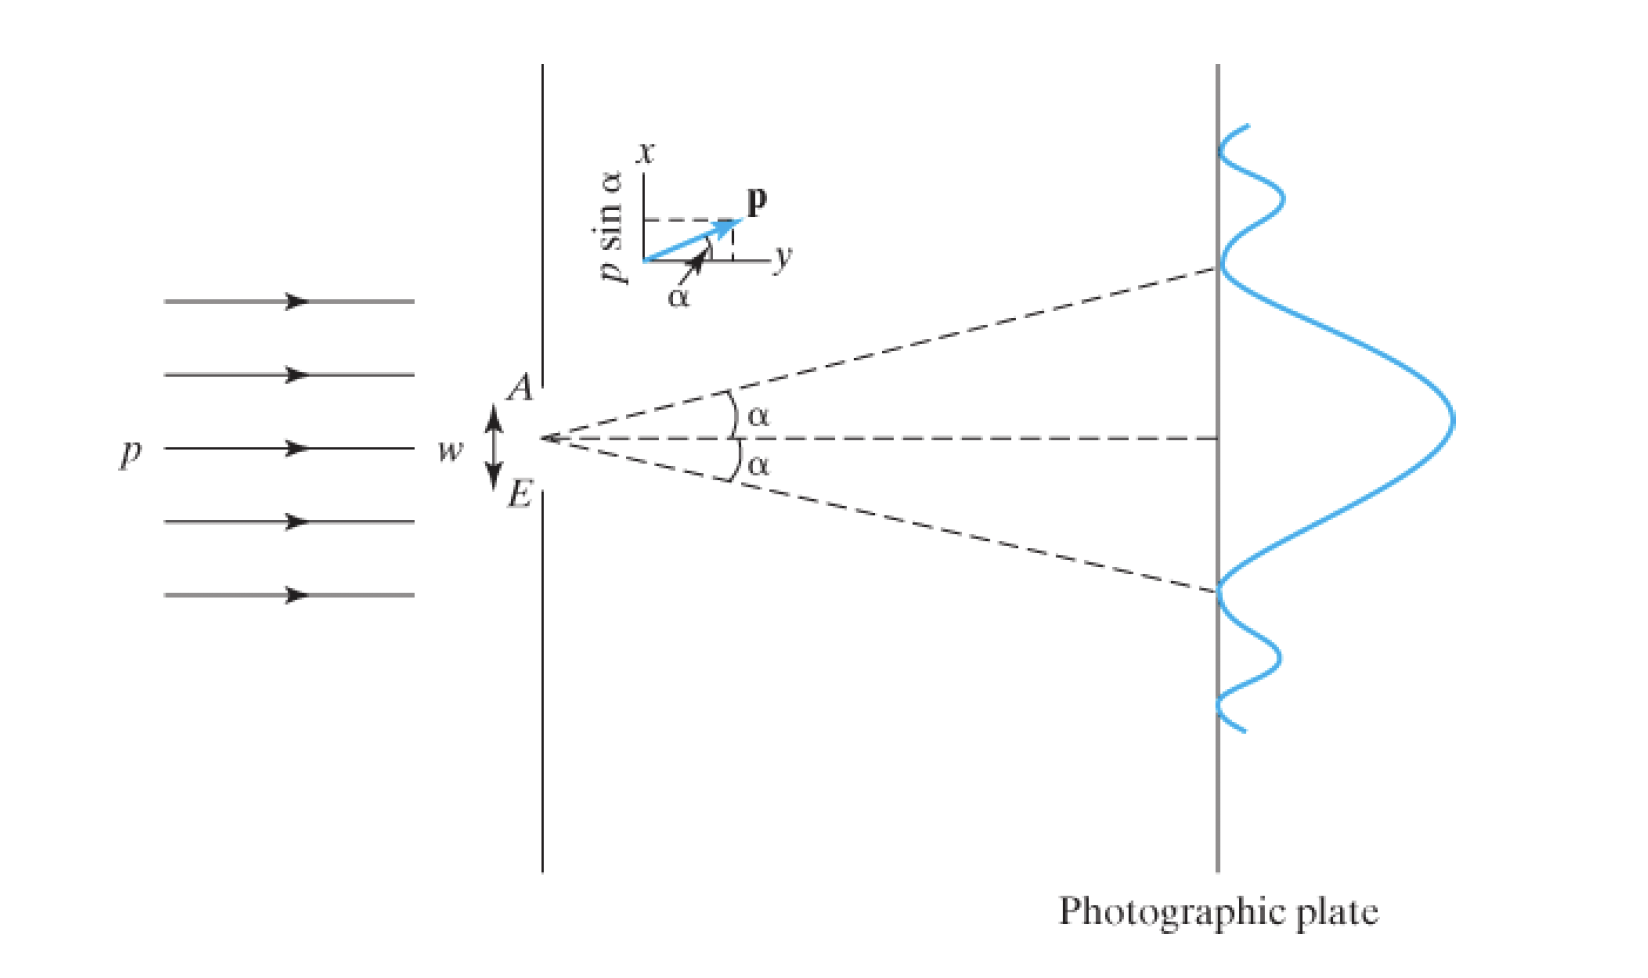
\includegraphics[width=0.8\textwidth]{/users/administrator/desktop/quantum chemistry/Figures/1.1.png}  % 图片路径
		\caption{\text{狭缝的电子衍射}}
		\label{fig:1.1}
	\end{figure}
	\begin{figure}[h!]
		\centering
		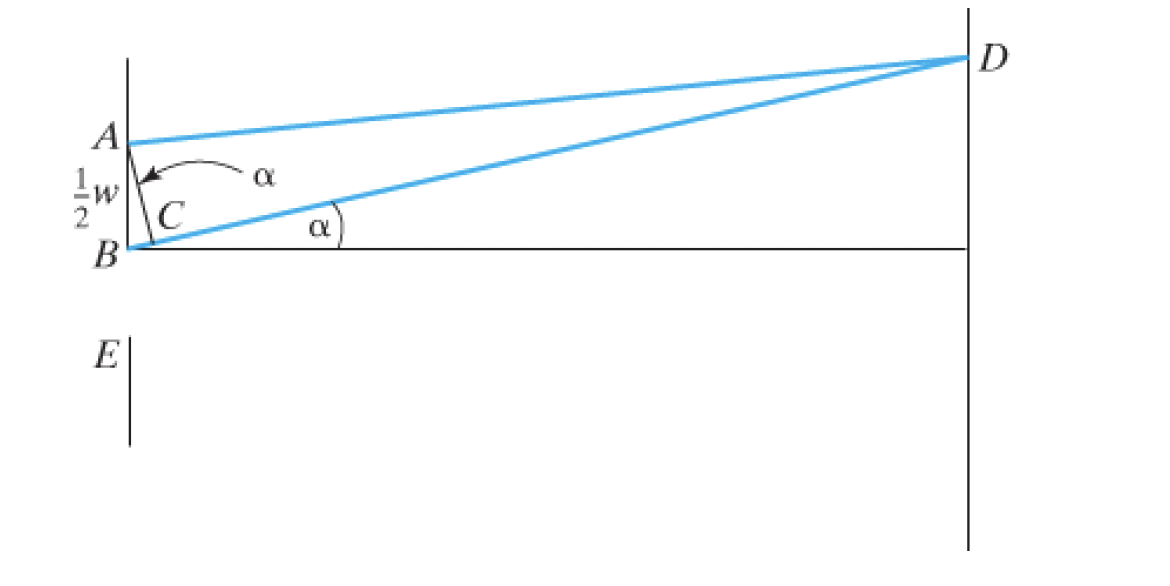
\includegraphics[width=0.6\textwidth]{/users/administrator/desktop/quantum chemistry/Figures/1.2.png}
		\caption{\text{计算一级衍射的最小值}}
		\label{fig:1.2}
	\end{figure}
	
	\indent 第一个衍射最小值出现的角度$\alpha$很容易计算。出现第一个最小值的条件是:通过狭缝上边缘的粒子和通过狭缝中心的粒子所经过的距离之差应等于$\frac{1}{2}\lambda$,其中$\lambda$是相关波的波长。这样,从狭缝顶部发出的波与从狭缝中心发出的波正好相位相反,它们相互抵消。从狭缝中点以下距离$d$处发出的波与从狭缝顶部以下距离$d$处发出的波相互抵消。在图 \ref{fig:1.2}中画出$AC$,使 $AD=CD$,则路径长度之差为$BC$。狭缝到屏幕的距离比狭缝宽度大。因此,$AD和$BD几乎平行,则$\angle ACB$基本上是直角,因此$\angle BAC = \alpha$ ,路径差$BC$就是$\frac{1}{2}w \sin \alpha$。 设$BC$等于$\frac{1}{2}\lambda$,我们就得到了$w\sin\alpha=\lambda$,公式\ref{eq:diffract equation on x} 就变成了$\Delta x \Delta p_x=p\lambda$,其中波长$\lambda$由德布罗意关系式$\lambda=h/p$给出,因此$\Delta x \Delta p_x=h$。由于不确定度尚未精确定义,因此使用等号并不合适。我们可以用 
	\begin{equation}
		\Delta x \Delta p_x \approx h
		\label{eq:uncertinty on x}
	\end{equation}
	来表示$x$方向上的不确定性,同时$p_x$具有与普朗克常数相当的的数量级。
	
	
	\section{含时薛定谔方程}
	
	\section{定态薛定谔方程}
	
	\section{概率}
	
	\section{复数}
	
	\section{单位}
	
	\section{微积分学}
	
	\section*{总结}

	\section*{习题}
	
	% ===== CHAPTER 2 =====
	\chapter{箱中粒子}
	\section{微分方程}
	The general solution to the linear homogeneous second-order differential equation:
	\begin{equation}
		y'' + py' + qy = 0
	\end{equation}
	is $y = c_1 e^{s_1 x} + c_2 e^{s_2 x}$ where $s_1$ and $s_2$ are roots of the auxiliary equation $s^2 + ps + q = 0$.
	
	\section{一维盒子中的粒子}
	The wavefunctions and energies are:
	\begin{align}
		\psi_n(x) &= \sqrt{\frac{2}{l}} \sin\left(\frac{n\pi x}{l}\right) \\
		E_n &= \frac{n^2 h^2}{8ml^2}, \quad n = 1,2,3,\ldots
	\end{align}

	
	\section{一维自由粒子}
	
	\section{矩形势井中的粒子}
	
	\section{隧穿}
	
	\section*{总结}
	
	\section*{习题}
	
	
	
	
	
	% ===== CHAPTER 3 =====
	\chapter{算符}
	\section{算符}
	
	\section{本征函数和本征值}
	An operator $\hat{A}$ satisfies:
	\begin{equation}
		\hat{A} \psi = a \psi
	\end{equation}
	where $a$ is the eigenvalue.
	
	\section{算符和量子力学}
	Key operators in quantum mechanics:
	\begin{align}
		\text{Position:} & \quad \hat{x} = x \\
		\text{Momentum:} & \quad \hat{p}_x = -i\hbar \pdv{x} \\
		\text{Hamiltonian:} & \quad \hat{H} = -\frac{\hbar^2}{2m} \nabla^2 + V(\mathbf{r})
	\end{align}
	
	\section{三维多粒子的薛定谔方程}
	
	\section{三维盒子中的粒子}
	
	\section{简并}
	
	\section{平均值}
	
	\section{波函数的约束条件}
	
	\section*{总结}

	\section*{习题}
	
	
	% ===== CHAPTER 4 =====
	\chapter{谐振子}
	\section{微分方程的幂级数解}
	
	\section{一维谐振子}
	
	\section{双原子分子的振动}
	
	\section{一维定态薛定谔方程的数值解法}
	
	\section*{总结}
	
	\section*{习题}
	
	% ===== CHAPTER 5 =====
	\chapter{角动量}
	\section{Simultaneous Specification of Several Properties}
	
	\section{向量}
	
	\section{单粒子系统的角动量}
	
	\section{角动量梯度算符法}
	
	\section*{总结}
	
	\section*{习题}
	
	% ===== CHAPTER 6 =====
	\chapter{氢原子}
	\section{单粒子中心力问题}
	
	\section{无相互作用的粒子和变量分离}
	
	\section{将双粒子问题简化为两个单粒子问题}
	
	\section{双粒子的刚性转子模型}
	
	\section{氢原子}
	
	\section{束缚态氢原子波函数}
	
	\section{类氢轨道}
	
	\section{塞曼效应}
	
	\section{径向薛定谔方程的数值解法}
	
	\section*{总结}
	
	\section*{习题}
	
	% ===== CHATPTER 7 =====
	\chapter{量子力学理论}
	\section{符号}
	
	\section{厄米算符}
	
	\section{用本征函数展开}
	
	\section{对易算符的本征函数}
	
	\section{宇称}
	
	\section{测量和态叠加}
	
	\section{坐标本征函数}
	
	\section{量子力学的基本假设}
	
	\section{测量和量子力学解释}
	
	\section{矩阵}
	
	\section*{总结}
	
	\section*{习题}
	
	% ===== CHAPTER 8 =====
	\chapter{变分法}
	\section{变分理论}
	
	\section{变分法的推广}
	
	\section{行列式}

	\section{联立线性方程组}
	
	\section{线性变分函数}
	
	\section{矩阵、本征值和本征向量}
	
	\section*{总结}
	
	\section*{习题}
	
	% ===== CHAPTER 9 =====
	\chapter{微扰理论}
	\section{微扰理论}
	
	\section{非简并微扰理论}
	
	\section{微扰理论求解基态氦原子}
	
	\section{能量简并的微扰理论}
	
	\section{久期方程的简化}
	
	\section{微扰理论求解第一激发态的氦原子}
	
	\section{含时微扰理论}
	
	\section{辐射和物质的相互作用}
	
	\section*{总结}
	
	\section*{习题}
	
	% ===== CHAPTER 10 =====
	\chapter{电子自旋和自旋-统计定理}
	\section{电子自旋}
	
	\section{自旋和氢原子}
	
	\section{自旋-统计定理}
	
	\section{氦原子}
	
	\section{Pauli不相容原理}
	
	\section{Slater行列式}
	
	\section{微扰理论求解基态锂原子}
	
	\section{变分法求解基态锂原子}
	
	\section{自旋磁矩}
	
	\section{电子自旋的梯度算符}
	
	% ===== CHAPTER 11 =====
	\chapter{多电子原子}
	\section{Hartree-Fock自洽场方法}
	
	\section{轨道和元素周期表}
	
	\section{电子相关}
	
	\section{角动量的叠加}
	
	\section{多电子原子的角动量}
	
	\section{自旋-轨道耦合}
	
	\section{原子哈密顿算符}
	
	\section{Condon-Slater规则}
	
	\section*{总结}
	
	\section*{习题}
	
	% ===== CHAPTER 12 =====
	\chapter{分子对称性}
	\section{对称元素和对称操作}
	
	\section{分子点群}
	
	\section*{总结}
	
	\section*{习题}
	
	% ===== CHAPTER 13 =====
	\chapter{双原子分子的电子结构}
	\section{Born-Oppenheimer近似}
	
	\section{双原子分子核的运动}
	
	\section{原子单位制}
	
	\section{氢分子离子}
	
	\section{H$_2^+$离子基态的近似解}
	
	\section{H$_2^+$离子激发态的分子轨道}
	
	\section{同核双原子分子的分子轨道构型}
	
	\section{双原子分子的分子光谱项}
	
	\section{氢分子}
	
	\section{价键理论求解H$_2$}
	
	\section{分子轨道理论和价键理论的比较}
	
	\section{同核双原子分子的分子轨道理论和价键理论波函数}
	
	\section{H$_2$分子的激发态}
	
	\section{双原子分子的自洽场方法波函数}
	
	\section{分子轨道理论处理异核双原子分子}
	
	\section{价键理论处理异核双原子分子}
	
	\section{价电子近似}
	
	% ===== CHAPTER 14 =====
	\chapter{分子量子力学理论}
	\section{电子概率密度}
	
	\section{偶极矩}
	
	\section{分子的Hartree-Fork方法}
	
	\section{Virial理论}
	
	\section{Virial理论和化学键}
	
	\section{Hellmann-Feynman理论}
	
	\section{静电力定理}
	
	\section*{总结}
	
	\section*{习题}
	
	% ===== CHAPTER 15 =====
	\chapter{分子的电子结构}
	\section{从头计算、密度泛函、半经验和分子力学方法}
	
	\section{多原子分子的分子光谱项}
	
	\section{自洽场方法、分子轨道理论求解多原子分子}
	
	\section{基函数}
	
	\section{自洽场方法、分子轨道理论求解H$_2$O分子}
	
	\section{布居数和键级}
	
	\section{分子静电势、分子表面和原子电荷}
	
	\section{离域分子轨道}
	
	\section{自洽场方法、分子轨道理论求解甲烷、乙烷和乙烯}
	
	\section{分子结构学}
	
	\section{构象搜寻}
	
	\section{分子振动频率}
	
	\section{热力学定律}
	
	\section{从头计算方法的量子化学程序}
	
	\section{进行从头计算}
	
	\section{快速Hartree-fock计算方法}
	
	\section{溶剂效应}
	
	\section*{习题}
	
	% ===== CHAPTER 16 =====
	\chapter{电子关联方法}
	\section{关联能}
	
	\section{组态相互作用}
	
	\section{多体微扰理论}
	
	\section{耦合簇方法}
	
	\section{密度泛函理论}
	
	\section{能量计算的复合方法}
	
	\section{扩散量子Monte Carlo法}
	
	\section{非共价相互作用}
	
	\section{NMR屏蔽常数}
	
	\section{碎裂法}
	
	\section{相对论效应}
	
	\section{价键理论求解多原子分子}
	
	\section{GVB(广义价键波函数)、VBSCF(价键自洽场)、BOVB(呼吸轨道价键)方法}
	
	\section{化学反应}
	
	\section*{习题}
	
	% ===== CHAPTER 17 =====
	\chapter{半经验和分子力学方法求解分子}
	\section{半经验分子轨道求解平面共轭分子}
	
	\section{Hückel分子轨道理论}
	
	\section{PPP方法}
	
	\section{一般的半经验分子轨道和密度泛函方法}
	
	\section{分子力学方法}
	
	\section{经验和半经验方法处理溶剂效应}
	
	\section{化学反应}
	
	\section{量子化学的未来}
	
	\section*{习题}
	
	
	
	
	
	
	% ===== APPENDIX =====
	\appendix
	\chapter*{附录}
	\section{Complex Numbers}
	A complex number $z = x + iy$ can be expressed as:
	\begin{equation}
		z = re^{i\theta}, \quad r = \sqrt{x^2 + y^2}, \quad \theta = \tan^{-1}(y/x)
	\end{equation}
	
	\section{Calculus Formulas}
	Key differentiation and integration formulas:
	\begin{align}
		\dv{x}(e^{ax}) &= ae^{ax} \\
		\int \sin(ax) \dd{x} &= -\frac{1}{a} \cos(ax) + C
	\end{align}
	
	% ===== BIBLIOGRAPHY =====
	\chapter*{参考文献}
	\begin{thebibliography}{9}
		\bibitem{levine} 
		Levine, I. N. (2014). \emph{Quantum Chemistry} (7th ed.). Pearson.
	\end{thebibliography}
	
	% ===== ANSWERS TO SELECTED PROBLEMS =====
	\chapter*{部分习题答案}
	
	
	% ===== INDEX =====
	\chapter*{索引}
	
\end{document}